% -----------------------------------------------
% Template for ISMIR Papers
% 2016 version, based on previous ISMIR templates

% Requirements :
% * 6+1 page length maximum
% * 2MB maximum file size
% * Copyright note must appear in the bottom left corner of first page
% (see conference website for additional details)
% -----------------------------------------------

\documentclass{article}
\usepackage{ismir,amsmath,cite}
\usepackage{graphicx}
\usepackage{color}
\usepackage[]{algorithm2e}
\usepackage{color}
\usepackage{multirow}
\usepackage{subfigure}
\usepackage[justification=centering]{caption}
\usepackage{epstopdf}
\usepackage{float} 

\usepackage{amssymb}
\usepackage[]{algorithm2e}
\usepackage{enumitem} 



% Title.
% ------
\title{Genre specific dictionaries for harmonic/percussive source separation}

% Note: Please do NOT use \thanks or a \footnote in any of the author markup

% Single address
% To use with only one author or several with the same address
% ---------------
%\oneauthor
% {Names should be omitted for double-blind reviewing}
% {Affiliations should be omitted for double-blind reviewing}

% Two addresses
% --------------
%\twoauthors
%  {First author} {School \\ Department}
%  {Second author} {Company \\ Address}

% Three addresses
% --------------
%\threeauthors
%  {First author} {Affiliation1 \\ {\tt author1@ismir.edu}}
%  {Second author} {\bf Retain these fake authors in\\\bf submission to preserve the formatting}
%  {Third author} {Affiliation3 \\ {\tt author3@ismir.edu}}

% Four addresses
% --------------
\fourauthors
  {Cl\'{e}ment Laroche} {Affiliation1 \\ {\tt author1@ismir.edu}}
  {Second author}{Affiliation2 \\ {\tt author2@ismir.edu}}
  {Third author} {Affiliation3 \\ {\tt author3@ismir.edu}}
  {Fourth author} {Affiliation4 \\ {\tt author4@ismir.edu}}

\begin{document}
%
\maketitle
%
\begin{abstract}
The abstract should be placed at the top left column and should contain about 150-200 words.
\end{abstract}
%
\section{Introduction}\label{sec:introduction}


\emph{Source separation} is field of ​​research that seeks to separate the components of an audio signal present in a record. Such separation has many applications in music : noise suppression \cite{boll1979suppression} (if a source is a noise) , up-mixing \cite{fitzgerald2011upmixing}(spatialization of the sources) or automatic transcription \cite{Bertin07} (it is easier to operate on single source). The task is difficult due to the complexity and the variability of the music mixtures. Most datasets used for Blind Source Separation (BSS) research are small in size and they do not allow for a thorough comparison of the algorithms. Using a larger database is crucial to benchmark the separation algorithms in order to obtain a true evaluation rather than particular case results. 

The large variety of audio signal can be classified into different musical genres \cite{tzanetakis2002musical}. Genres are labels created and used by humans for categorizing and describing music. They have no strict definitions and boundaries but particular genre share certain characteristics typically related to the instrumentation, rhythmic structure, and pitch content of the music and the resemblance between two pieces of music have been used to perform chord transcription \cite{ni2012using,lee2008acoustic} or for downbeat detection \cite{hockman2012one}. Finally when the genre information is not available, it is possible to perform automatic genre classification \cite{li2003comparative}.




In the context of BSS, Non-negative Matrix Factorization (NMF) is a widely used method for source separation. The goal of NMF is to approximate a data matrix $V \in \mathbb{R}_{+}^{n \times m} $ as $V \approx \tilde{V} = WH$ with $W \in \mathbb{R}_{+}^{n \times k}$, $H \in \mathbb{R}_{+}^{k \times m}$ and where $k$ is the rank of factorization \cite{lee99}. In audio signal processing, the input data is usually a Time-Frequency (TF) representation such as a short time Fourier transform (STFT) or a constant-Q transform spectrogram. Blind source separation is a difficult problem and the plain NMF decomposition does not provide satisfying results. To perform a satisfying results, it is necessary to exploit various features that make each sources distinguishable from one another. 
Supervised algorithms in the NMF framework exploit training data or prior information in order to guide the decomposition process. For example information from the scores or from midi signals \cite{EwertM12} can be used to initialize the learning process. The downside of this approach is that it requires well organized prior information that is not always available. Another supervised method consists in performing prior training on specific databases. For example a dictionary matrix $W_{train}$ is learned from a big database in order to separate an instrument \cite{jaureguiberry2011adaptation,wudrum}. A common method to build a dictionary for NMF is to perform a decomposition on a large training set. After the convergence, the $W$ matrix from the decomposition is used as the dictionary matrix $W_{train}$ in the separation \cite{jaureguiberry2011adaptation}. Another method is detailed in \cite{wudrum}, a dictionary matrix is created by extracting template spectra from isolated drum samples. The dictionary is then used in a NMF decomposition to perform drum transcription. This method requires minimum tuning from the user. However, the dictionary should match the target instrument for satisfying performances. 


In this paper, we focus on the task of harmonic/percussive source separation (HPSS) using the method developed in \cite{laroche2015structured}. We adapt the method to be used with a drum dictionary to extract the percussive instruments. This method is explained in detail in the preprint. 
The problem of using a fixed dictionary matrices is that within a database, the same instrument can sound differently depending on the recording condition and post processing treatment. In order to represent correctly one instrument, ones can decide to learn a dictionary on a large database. However, the problem of over-fitting the data exist. In order to overcome this problem and to build effective dictionaries we decided to use genre specific training data. As they share similar features genre specific information can provide an insight on the structure of the audio signal.
The main contribution of this article is that we developed a genre specific method to build a drum NMF dictionary that obtains consistent results on a HPSS task. By using genre specific dictionary we were able to improve the separation score compared to a universal dictionary. 
 


\section{Structured projective NMF (SPNMF)}
\label{sec:SPNMF}

In this section we present our semi-supervised algorithm for harmonic/percussive source separation.

\subsection{Presentation of the orthogonal and projective NMF}\label{subsec:PNMF}


The aim of PNMF is to find a non negative projection matrix $P \in \mathbb{R}_{+}^{n \times n}$ such that $V \approx \tilde{V} = PV$. In~\cite{yuanOja2005} Yuan \& al. propose to seek $P$ as an approximative projection matrix under the form $P = WW^{T}$ with $W \in \mathbb{R}_{+}^{n \times k}$ with $ k \leqslant n $. The PNMF problem reads : 
\begin{equation}\label{EqPnmf}
\min_{W \geqslant 0} ||V - WW^{T}V||^2 
\end{equation}

PNMF is similar to the NMF problem and can be simply obtained by replacing the activation matrix $H$ by $W^TV$. It is shown in~\cite{YangOja10} that the PNMF gives a much sparser decomposition than NMF.

Another very similar approach is the ONMF~\cite{choi}. It consists in solving the following problem: 
\begin{align}
\min_{W \geqslant 0, H \geqslant0} ||V - WH||^2 \quad   \text{s.t}.\quad W^{T}W=I_{k} 
\end{align}%
In this method, orthogonality between nonnegative basis functions is enforced during the optimization process. In theory, it seems that PNMF and ONMF lead to similar decompositions, as the $W$ matrix estimated by PNMF is almost orthogonal (i.e., $\|W^{T}W-I_{k}\|^{2}$ is small). However in practice, enforcing the orthogonality between the base at every iteration is a constraint too strong to decompose audio signal~\cite{laroche2015structured}. 

The sparsity of the dictionary matrix is an interesting property for the decomposition of audio signals and especially for the decomposition of harmonic instruments with very localized harmonic spectra. Contrary to the NMF, the sparsity of PNMF and is an inherent features of the decomposition. These key properties of PNMF motivated us to decompose the harmonic instruments with the orthogonal basis functions.


\subsection{Principle of the SPNMF}

The orthogonal basis functions of PNMF are not flexible enough to decompose a complex audio signal. As stated in~\cite{canadas2014percussive}, harmonic instruments have sparse basis functions whereas percussive instruments have much flatter spectra. As the columns of $W$ are orthogonal, when two sources overlap in the Time-Frequency (TF) plane only one basis function will represent the mixture which is not adequate for efficient separation. To overcome this problem, we propose to add a standard NMF decomposition term to the PNMF. We can expect that most of the harmonic components will be represented by the orthogonal part while the percussive ones will be the regular NMF components. Using a similar model as in our preliminary work~\cite{laroche2015structured}, let $V$ be the magnitude spectrogram of the input data. The model is then given by
\begin{equation} \label{Cfunction}
V \approx \tilde{V}= V_H + V_{P},
\end{equation}
with $V_P$ the spectrogram of the percussive part and $V_H$ the spectrogram of the harmonic part. $V_H$ is approximated by the PNMF decomposition while $W_P$ is decomposed by NMF components as :
\begin{equation}
V \approx \tilde{V}= W_{H}W_{H}^{T}V + W_{P} H_{P}.
\end{equation}
The data matrix is approximated by an almost orthogonal sparse part that codes the harmonic instruments $V_H = W_HW_H^T V$ and a non constrained NMF part that codes the percussive instruments $V_P = W_PH_P$. However, a fully unsupervised SPNMF model does not allow for a satisfying harmonic/percussive source separation~\cite{laroche2015structured}. To alleviate this problem, we use here a fixed drum dictionary $W_p$ in the percussive part of the SPNMF.



\subsection{Algorithm Optimization}

In order to obtain such a decomposition, we can use a measure of fit $D(x|y)$ between the data matrix $V$ and the estimated matrix $\tilde{V}$. $D(x|y)$ is a scalar cost function and in this article, we use the Itakura Saito (IS) divergence.



The SPNMF model gives the cost function : 
\begin{equation}\label{InitCost}
\min_{W_H,W_P,H_P \geq 0} D(V|W_{H}W_{H}^{T}V + W_{P} H_{P})  
\end{equation}

A solution of this problem can be obtained by iterative multiplicative update rules following the same strategy as in~\cite{yuanOja2005,Lee01algorithmsfor} which consists in splitting the gradient with respect to (wrt) one variable (here $W_H$ for exemple) $\nabla_{W_H} D(V|\tilde{V})$ in its positive $[\nabla_{W_H} D(V|\tilde{V})]^{+}$ and negative parts $[\nabla_{W_H} D(V|\tilde{V})]^{-}$.
The multiplicative updates for SPNMF are then given by: 
$$W_{H} \leftarrow W_{H} \otimes \frac{ [\nabla_{W_H} D(V|\tilde{V})]^{-} }{[\nabla_{W_H} D(V|\tilde{V})]^{+}}, $$
where $\otimes$ is the Hadamard product or element-wise product. The SPNMF algorithm with a fixed dictionary matrix is:
 
\begin{algorithm}[h]
 Input: $V \in \mathbb{R}_{+}^{m \times n} $
 Output: $W \in \mathbb{R}_{+}^{m \times k}$, $W_{train} \in \mathbb{R}_+^{m \times e}$ and $H \in \mathbb{R}_{+}^{e \times n}$
 Initialization\;
 \While{$i \leq$ number of iterations}{
	$H_{P} \leftarrow H_{P} \otimes \frac{ [\nabla_{H_P} D(V|\tilde{V})]^{-} }{[\nabla_{H_P} D(V|\tilde{V})]^{+}}$
	

	$W_{H} \leftarrow W_{H} \otimes \frac{ [\nabla_{W_H} D(V|\tilde{V})]^{-} }{[\nabla_{W_H} D(V|\tilde{V})]^{+}}$
	 \vspace{0.2cm}
	 	
	$i=i+1$ 
 }
 $ X_P = W_{train}H_P $ and
 $ X_H = W_HW_H^TV $ 
  
\vspace{0.2cm}
 \caption{SPNMF with the drum dictionary matrix.}\label{AlgoDictionary}
\end{algorithm}




 
\subsection{Signal reconstruction}

The percussive signal $x_p(t)$ is synthesized using the magnitude percussive spectrogram $X_P = W_PH_P$. To reconstruct the phase of the percussive part, we use a generalized Wiener filter~\cite{liutkus2015generalized} to create a percussive mask as:
\begin{equation}
\mathcal{M}_P = \frac{X_P^2}{X_M^2 + X_P^2}.
\end{equation} 
To retrieve the percussive signal as, 
\begin{equation}
x_p(t) = InverseSTFT(\mathcal{M}_P \otimes X).
\end{equation}
Where $X$ is the complex spectrogram of the mixture.
Similarly for the harmonic part, we obtain:
\begin{equation}\label{percuweiner}
\mathcal{M}_H = \frac{X_H^2}{X_M^2 + X_P^2},
\end{equation}
and:
\begin{equation}
x_h(t) = InverseSTFT(\mathcal{M}_H \otimes X).
\end{equation}




\section{Construction of the dictionary}



\subsection{Optimal size for the dictionary}\label{optimalsize}

The first step to build a NMF drum dictionary is to select the rank of factorization. We run different tests on the public SiSec database from~\cite{SiSec10}. It is composed of polyphonic real-world music excerpts and each music signal contains percussive, harmonic instruments and vocals. The duration of the four recording is ranging from $14$ to $24$~s. The goal is to perform an harmonic/percussive decomposition. Following~\cite{canadas2014percussive}, we will not consider the vocal part and we will build mixture signals only from the percussive and harmonic instruments. All the signals are sampled at $44.1kHz$. We compute the STFT with a and $2048$ sample-long Hann window with a $50\%$ overlap.

The drum signal used for the training comes from the database \cite{gillet2006enst} and the signal is around $3$min long. We used $14$ files from the database were the drummer is playing a \emph{drum phrase}. We compute an NMF decomposition with different rank of factorization ($k=12$, $k=50$, $k=100$, $k=500$, $k=1000$ and $k=2000$) on the drum signal alone to obtain $6$  drum dictionaries.
The dictionaries are then used to perform a HPSS on the four songs of the SiSEC database. The results are displayed on figure \ref{dictsize}.

\begin{figure}[h]

  \centering 
  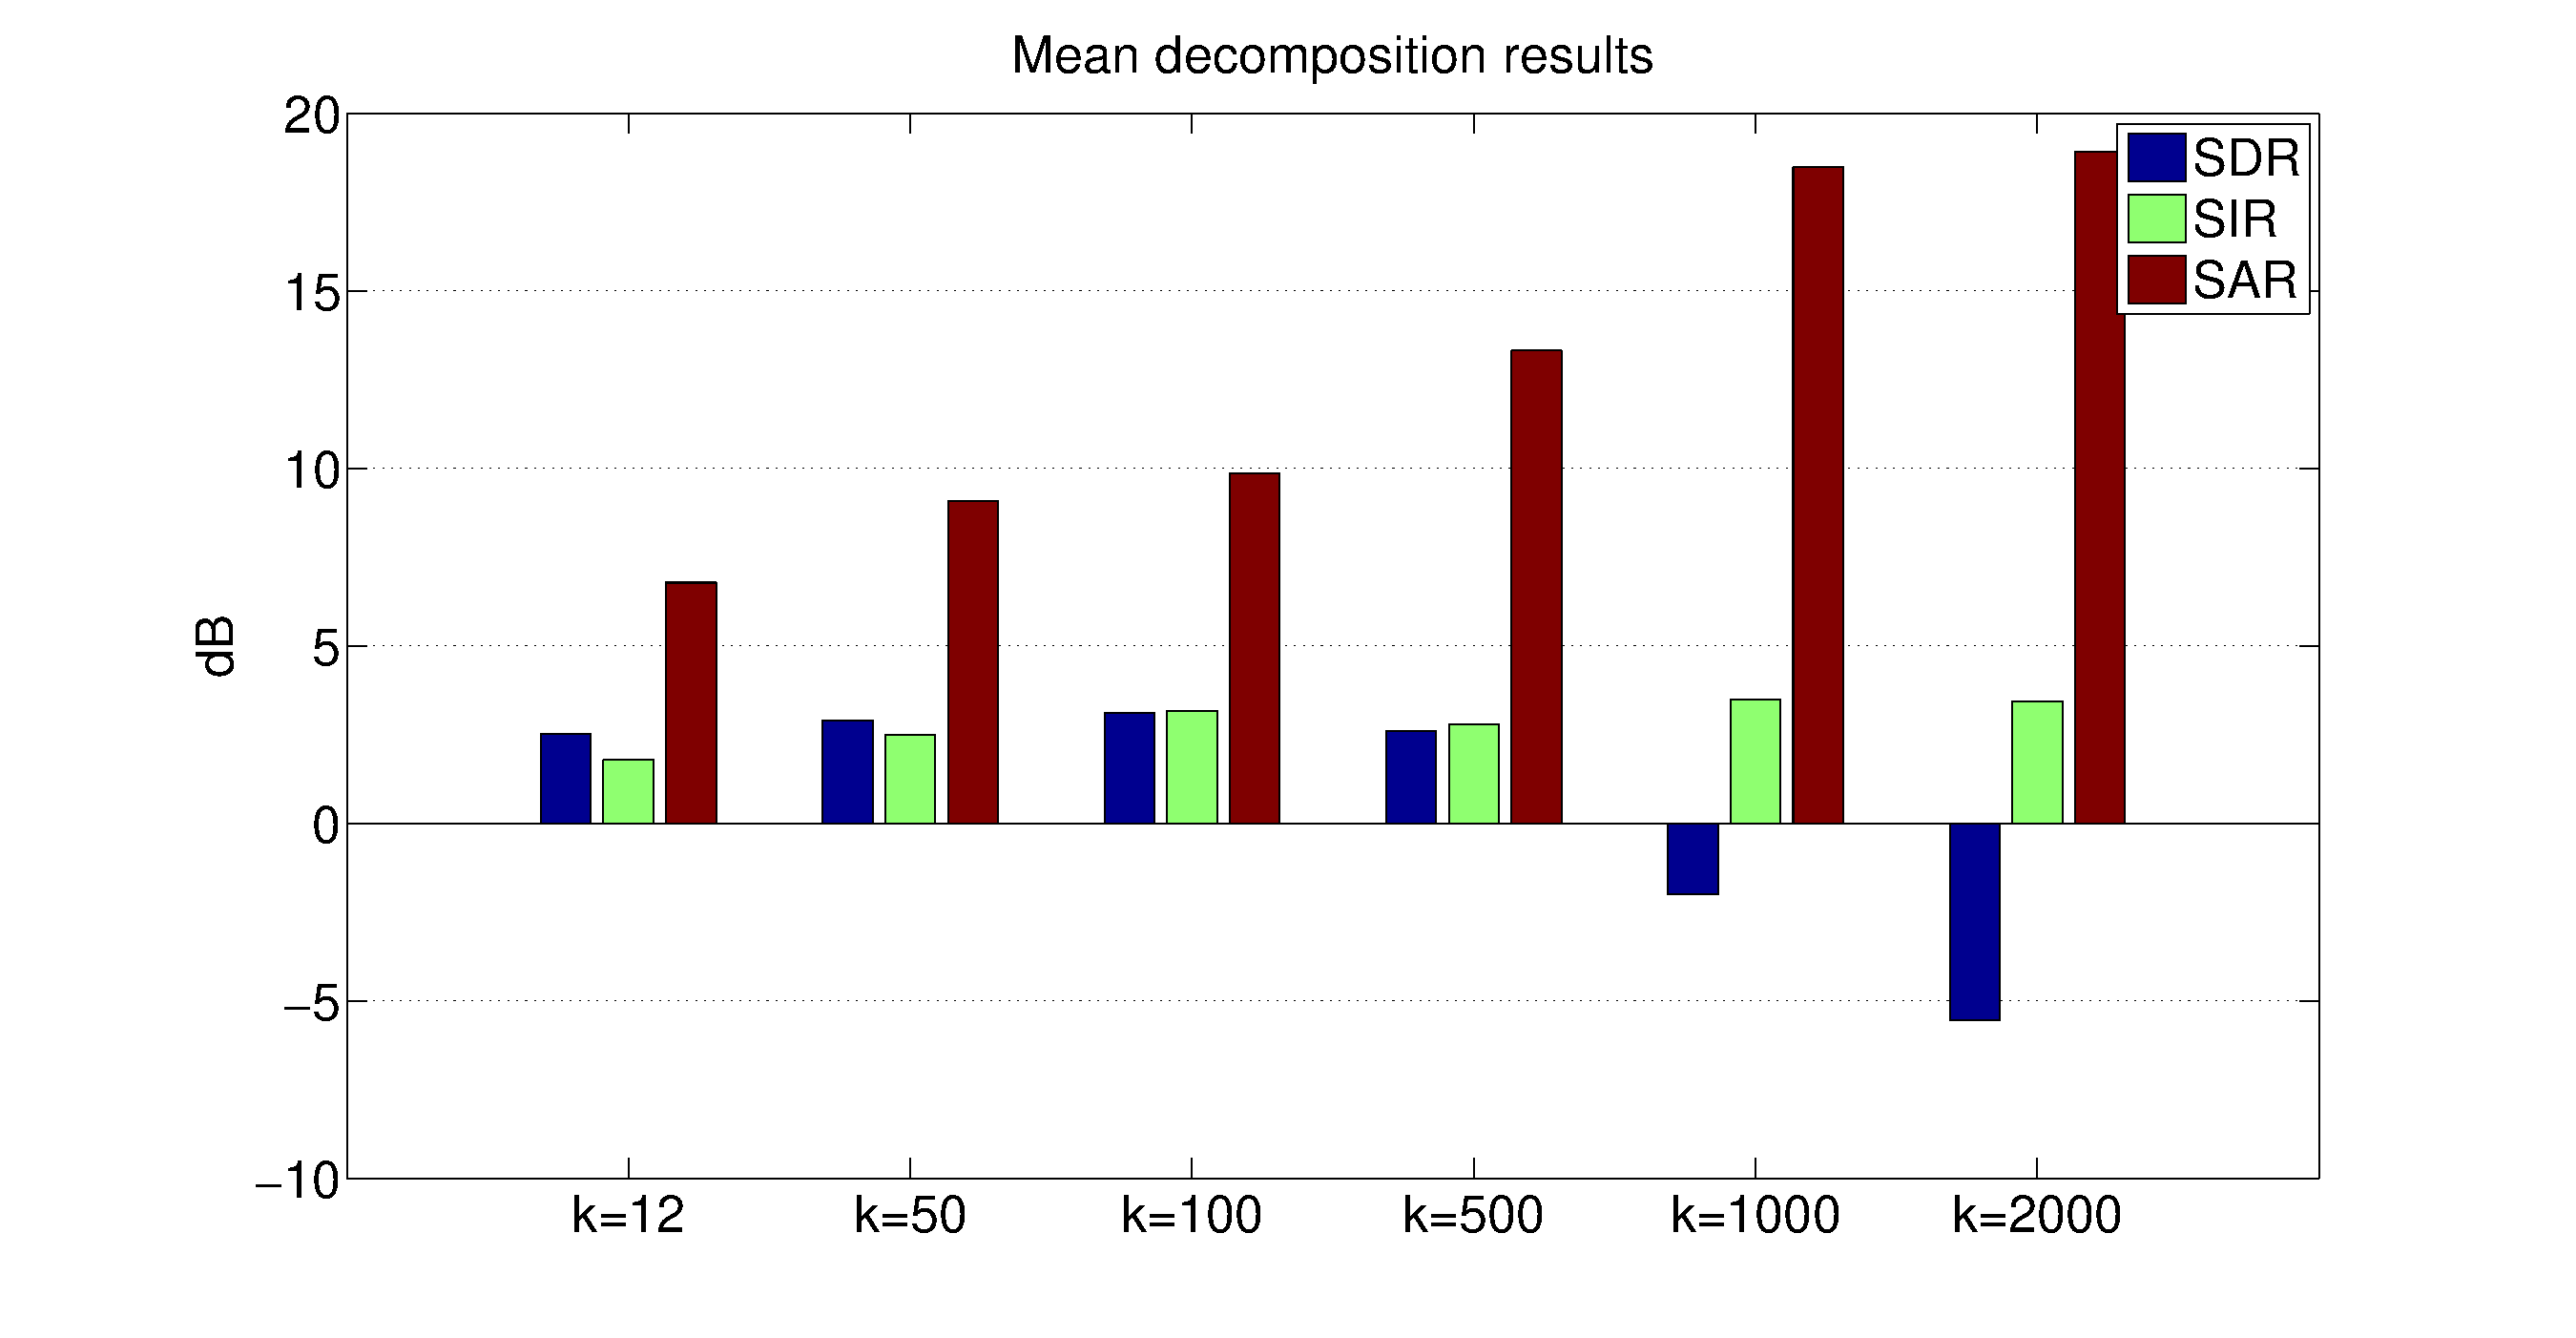
\includegraphics[width=9cm]{figs/AllDictSizeISMIR.eps}
%  \vspace{2.0cm}
  \caption{\label{dictsize} Average results on the SiSec database.}
  
\end{figure}
 

\subsection{Database}\label{database}

The dataset is taken from medley-dB \cite{bittner2014medleydb}, it is composed of polyphonic real-world music excerpts. It has $122$ music signals and $87$ of them contain percussive instruments, harmonic instruments and vocals. The signals that do not contain a percussive part are not part of the evaluation. We will be using the song of the genre, \emph{Classical} ($8$ songs), \emph{Singer/Songwriter} ($17$ songs), \emph{Pop} ($10$ songs), \emph{Rock} ($20$ songs), \emph{Jazz} ($11$ songs), \emph{Electronic/Fusion} ($13$ songs) and \emph{World/Folk} ($6$ songs). Because the notion of genre is quite subjective, the medley-dB database uses general genre labels. These labels should not be considered to be "precise" genre labels. There are many instances where a song could have fallen in multiple genres, and the choices were made so that each genre would be as acoustically homogeneous as possible. As we are only working with the instrumental part of the song "Pop" label (for example) are similar to the "Singer/Songwriter".
We use $3$ song of each genre to use as a training database. The songs used for the training part are not part of the evaluation. To compare the genre specific dictionary, we build a non specific/universal dictionary that is build using a half song of each genre. The files selected are:


\begin{table} 
	\centering 
   \begin{tabular}{|l|l|}
   	\hline   
Classical  & JoelHelander Definition \\
 & MatthewEntwistle AnEveningWithOliver \\
 & MusicDelta Beethoven \\
\hline
Electronic/Fusion & EthanHein 1930sSynthAndUprightBass \\
 & TablaBreakbeatScience Animoog \\
 & TablaBreakbeatScience Scorpio \\
\hline
Jazz & CroqueMadame Oil \\
 & MusicDelta BebopJazz \\
 & MusicDelta ModalJazz \\
\hline
Pop &  DreamersOfTheGhetto HeavyLove \\
 & NightPanther Fire \\
 & StrandOfOaks Spacestation \\
\hline
Rock & BigTroubles Phantom \\
 & Meaxic TakeAStep \\
 & PurlingHiss Lolita \\
\hline
Singer/Songwriter	& AimeeNorwich Child \\
 & ClaraBerryAndWooldog Boys \\
 & InvisibleFamiliars DisturbingWildlife \\
\hline
World/Folk & AimeeNorwich Flying \\
 &KarimDouaidy Hopscotch \\
 & MusicDelta ChineseYaoZu\\
\hline
Non specific & JoelHelander Definition \\
 & TablaBreakbeatScience Animoog \\
 & MusicDelta BebopJazz \\
 & DreamersOfTheGhetto HeavyLove \\
 &  BigTroubles Phantom \\
 & AimeeNorwich Flying \\
 &  MusicDelta ChineseYaoZu\\
 \hline

  
\end{tabular} 
\caption{\label{trainingdata} Song selected for the training database.}

\end{table}





\subsection{Genre specific dictionaries}

The NMF model is:
\begin{equation}
V \approx \tilde{V} = WH.
\end{equation}
If $V$ is the power spectrum of a drum signal, The matrix $W$ is a {\em dictionary} or a set of {\em patterns} that codes the frequency information of the drum. Building a dictionary specific to an instrument that performs well on a large database is a complicated problem. Here we build genre specific drum dictionary using the medley-dB database. Using dictionary specific to the genre of music allows us to have smaller dictionaries that a more specific to the signal to decompose. It grants us lower computation time and better separation score
The dictionary are build has follow. For every genre specific database of the training database, we perform and NMF with $k=300$ on the drum signals (with the results from Section \ref{optimalsize}, we choose $k=100$ per song for the NMF).

\begin{table}
   
	\centering 
   \begin{tabular}{|l|l|}
\hline   
Genre & Length(min)\\
\hline
Classical  & 22.06 \\
\hline
Electronic/Fusion & 18.66\\
\hline
Jazz & 10.96\\
\hline
Pop &  12.53 \\
\hline
Rock & 11.43\\
\hline
Singer/Songwriter & 9.36\\
\hline
World/Folk & 9.53\\
\hline
Non Specific & 11.03\\
\hline
  
\end{tabular} 
\caption{\label{lengthDict} Length of the genre specific database.}
\end{table}


\section{Results}

In this section we present the results of the algorithm with the genre specific dictionaries on the Medley-dB database.




% For bibtex users:
\bibliography{reference}

% For non bibtex users:
%\begin{thebibliography}{citations}
%
%\bibitem {Author:00}
%E. Author.
%``The Title of the Conference Paper,''
%{\it Proceedings of the International Symposium
%on Music Information Retrieval}, pp.~000--111, 2000.
%
%\bibitem{Someone:10}
%A. Someone, B. Someone, and C. Someone.
%``The Title of the Journal Paper,''
%{\it Journal of New Music Research},
%Vol.~A, No.~B, pp.~111--222, 2010.
%
%\bibitem{Someone:04} X. Someone and Y. Someone. {\it Title of the Book},
%    Editorial Acme, Porto, 2012.
%
%\end{thebibliography}

\end{document}
